% Chapter Template

\chapter{Introduction} % Main chapter title

\label{Chapter1} % Change X to a consecutive number; for referencing this chapter elsewhere, use \ref{ChapterX}

\lhead{Chapter 1. \emph{Introduction}} % Change X to a consecutive number; this is for the header on each page - perhaps a shortened title

%----------------------------------------------------------------------------------------
%	SECTION 1
%----------------------------------------------------------------------------------------

\section{Voice Activity Detection}

Voice Activity Detection (VAD) is a problem of separating parts of an audio recording which contain the presence of human voice from those which are only comprised of silence or the background noise. VAD is a trivial task in recordings which have high signal-to-noise (SNR) ratios, in which voice can be distinguished from noise simply by computing the short-time energy of all frames and setting an appropriate threshold for their classification. However, in real applications, the signal is almost always contaminated by some level of background noise which makes the VAD's performance to drop. VAD decision is especially difficult for the unvoiced phonemes \cite{Kondoz} whose spectrum contains no periodicity and is often similar to the one of white noise \cite{Michaelis}. \medskip

There has been an active research in the VAD area from as early as 1975, when Rabiner and Sambur \cite{RabinerSambur} proposed a VAD algorithm (then referred to as "algorithm for determining the endpoints of isolated utterances") based on the aforementioned short-time energy and the zero-crossing rate. This approach worked reasonably well for signals with SNR ratio on the order of 30 dB, however since then there has been a need for much better performance, including applications where algorithm robustness has to be achieved even at negative SNRs.

%----------------------------------------------------------------------------------------
%	SECTION 2
%----------------------------------------------------------------------------------------

\section{Applications}

VAD is often a first step in many signal processing applications including speech recognition \cite{RamirezGorriz}, speech coding \cite{Sohn}, speech enhancement \cite{Park} or noise estimation \cite{RamirezGorriz}. \medskip

In Automatic Speech Recognition (ASR), it is important to first extract the voice-active parts of a signal and then pass them to the actual recognition module. This procedure increases both the accuracy of the ASR system as well as its speed, since the recognition task is not performed on the parts of the signal which do not contain speech. An example structure of a ASR system which uses VAD module is presented in Figure \ref{fig:ASRVAD} \cite{RamirezGorriz}. For this application, it is most important for the VAD module to be able to identify all speech segments, even if some of the returned frames are false positives. Typically, there is a trade-off in VAD performance which can be characterised as maximising the precision of the VAD decisions while keeping the recall at a high rate.\medskip

\begin{figure}[htbp]
	\centering
		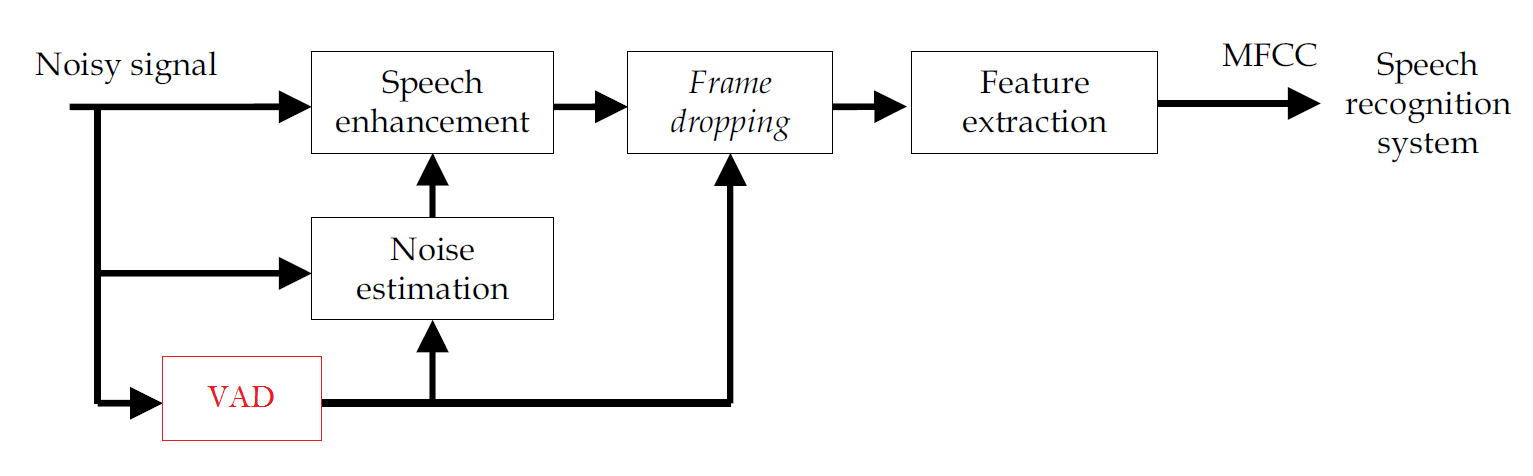
\includegraphics[width=1\columnwidth]{Figures/ASRVAD.png}
		\rule{34em}{0.5pt}
	\caption[Block diagram of an ASR system which uses VAD as the first processing step]{Block diagram of an ASR system which uses VAD as the first processing step \cite{RamirezGorriz}}
	\label{fig:ASRVAD}
\end{figure}

Variable-rate speech coding techniques and discontinuous transmission (DTX) \cite{GSMControl} systems also benefit from robust Voice Activity Detection. For DTX, 